
We saw in the last chapter that we need some way to provide for
\emph{disciplined} interaction between threads, to avoid threads interfering
with one another.  In this book, we will see three basic ways to achieve this:
message passing, monitors and semaphores.  At a higher level of abstraction,
we will also see how to use concurrent datatypes.

We will start with message passing.  In my opinion, it is the most intuitive
approach: one thread can send a message to another thread.  
In addition, message passing is  necessary for distributed computing, and also
works well with loosely coupled systems.  

A downside is that message passing tends to be slower than other approaches,
because there is an overhead in the sending and receiving of messages.
However, it is a good paradigm to start with, to get used to thinking about
concurrent programs.

The basic idea is that programs are composed of components, which might be
either threads (i.e.~sharing an address space) or processes (with distinct
address spaces, possibly on different computers).  These processes communicate
only by sending and receiving messages over \emph{channels}.  In this book, we
will be dealing with threads; but the same techniques can be used with
processes. 

%%%%%

\section{Channels}

Think of a channel as a directional wire.  Messages are sent at one end, and
received at the other end. 

%% \item At one end there is an output port, at the other an input port.
%% %
%% \begin{center}
%% \begin{tikzpicture}
%% \draw (0,0) node[draw] (sender) {\scalashape chan!v};
%% \draw (4.5,0) node[draw] (receiver) {\scalashape chan?()};
%% \draw[->] (sender) -- 
%%   node[above,near start]{\small outport} 
%%   node[above,near end]{\small inport} (receiver);
%% \end{tikzpicture}
%% \end{center}

%% \item Values sent at the outport end (using |chan!v|) are received at the
%%   inport end (using |chan?()|), in the same order.

%% \item
%% Channels can be either synchronous or asynchronous; we will use a mix in this
%% course.
%% \end{itemize}
%% \end{slide}

%%%%%

In SCL, \SCALA{Chan[A]} is the type of channels that pass data of
type~\SCALA{A}.  This has two concrete subtypes: |SyncChan[A]|, of synchronous
channels; and |BuffChan[A]|, of buffered (or asynchronous) channels.  We will
start by describing synchronous channels, and later describe buffered
channels. 

The command
\begin{scala}
  val chan = new SyncChan[A]
\end{scala}
defines |chan| to be a synchronous channel passing data of type~|A|.  Then the
command 
\begin{scala}
  chan!v
\end{scala}
sends the value \SCALA{v} on \SCALA{chan}.  The expression
\begin{scala}
  chan?()
\end{scala}
receives a value from~\SCALA{chan} and returns it.  The communication is
\emph{synchronous}: whichever part is executed first waits for the other; both
then proceed.  Thus the send and receive appear to take place at the same
time.  

%%%%%

For example, the following program prints the number 42 (in a round-about
way): 
\begin{scala}
  val chan = new SyncChan[Int]
  run(thread{ chan!42 } || thread{ println(chan?()) }) 
\end{scala}
%
This runs two threads: the first thread sends 42 on the channel; the second
thread receives a value on the channel, and prints it.

%%%%%

As another example, here's a thread that inputs values from the channel
\SCALA{in}, and outputs them on the channel~\SCALA{out}:
%
\begin{scala}
def copy[A](in: SyncChan[A], out: SyncChan[A]) = thread{
  while(true){ val x = in?(); out!x }
}
\end{scala}
%
(The function that creates the thread is parameterised by the channels, and by
the type~|A| of those channels.)
%
We could have written the body of \SCALA{copy} as simply:
\begin{scala}
  while(true) out!(in?()) 
\end{scala}
Note that in both forms, the communication on |in| can proceed even if no
thread is yet ready to receive on |out|.

%%%%%

A channel is simply an \SCALA{InPort} (something from which threads can
receive) and an \SCALA{OutPort} (something on which threads can send).  A
channel is composed of an |InPort| and an |OutPort|.
Note that the terminology ``|InPort|'' and ``|OutPort|'' refer to the point of
view of \emph{threads}, not channels: a thread receives values in on an
|InPort|, and sends values out on an |OutPort|; however, a value is put into a
channel on an |OutPort|, and passed out on an |InPort|.

Figure~\ref{fig:channel-types} outlines the relevant types.  (The definition
of |Chan[A]| uses multiple inheritance: it inherits definitions from both
|InPort[A]| and |OutPort[A]|.)  The types \SCALA{InPort[A]} and
\SCALA{OutPort[A]} can be abbreviated as \SCALA{??[A]} and~\SCALA{!![A]}.

%%%%%%

\begin{figure}
\begin{scala}
package ox.scl.channel

trait InPort[A]{ def ?(): A; ... }
        
trait OutPort[A]{ def !(value: A): Unit; ... }
  
trait Chan[A] extends InPort[A] with OutPort[A]{ ... }

class SyncChan[A] extends Chan[A]{...} 
\end{scala}
\caption{Outline of the types of channels.}
\label{fig:channel-types}
\end{figure}

%%%%%

The earlier function \SCALA{copy} uses only the \SCALA{InPort} of \SCALA{in}
and the \SCALA{OutPort} of \SCALA{out}.  We therefore could have written the
definition as:
%
\begin{scala}
def copy[A](in: ??[A], out: !![A]) = thread{ 
  while(true) out!(in?()) 
}
\end{scala}
%
This signature makes clear what the thread does with each channel, and so
helps with documentation (the names of the channels also help).  In addition,
this style provides some  type safety: if, for example, the code tries to send
on~|in|, the compiler will give a type error. 

%%%%%%%%%%%%%%%%%%%%%%%%%%%%%%%%%%%%%%%%%%%%%%%%%%%%%%%%%%%%

\section{Example: printing multiples of four}

We now consider a slightly larger example, which is an instance of a paradigm
known as \emph{fine-grained concurrency}: the system is built from several
small components which are composed in parallel.  It is not a very efficient
--- or even sensible --- way to create real programs.  We include such
examples here as they are a good way to get used to thinking about
concurrency, where multiple components work together, while keeping the
quantity of code small.  Also, such a programs could be thought of as a model
of an electronic circuit, with components implemented in hardware and wired
together.

The program appears in Figure~\ref{fig:Mults4}. The overall effect is to print
the multiples of four.

The function |console(in)| defines a component that repeatedly reads a value
from \SCALA{in} and writes it to standard output.  The function
\SCALA{nats(out)} defines a component that sends the natural numbers, in
order, on \SCALA{out}.  The function \SCALA{alts(in, out)} defines a component
that copies alternate values read from \SCALA{in} to \SCALA{out}.

%%%%%

\begin{figure}
\begin{scala}
object Mults4{
  def console[A](in: ??[A]) = thread{ while(true) println(in?()) }

  def nats(out: !![Int]) = thread{ 
    var n = 0; while(true){ out!n; n += 1 }
  }

  def alts[A](in: ??[A], out: !![A]) = thread{ 
    while(true){ out!(in?()); in?() } 
  }

  def system = {
    val x1, x2, x4 = new SyncChan[Int]
    nats(x1) || alts(x1, x2) || alts(x2, x4) || console(x4)
  }

  def main(args: Array[String]) = run(system)
}
\end{scala}
\caption{Printing multiples of four.}
\label{fig:Mults4}
\end{figure}

%%%%%

The definition of |system| creates appropriate channels and puts the
components together as illustrated below.
%
\begin{center}
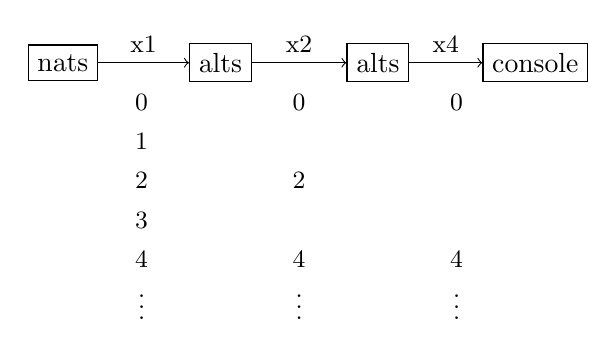
\begin{tikzpicture}
\draw (0,0) node[draw] (nats) {\scalashape nats};
\draw (nats)++(2,0) node[draw] (alts1) {\scalashape alts};
\draw[->] (nats) -- node[above]{\small\scalashape x1} (alts1);
\draw (alts1)++(2,0) node[draw] (alts2) {\scalashape alts};
\draw[->] (alts1) -- node[above]{\small\scalashape x2} (alts2);
\draw (alts2)++(2,0) node[draw] (console) {\scalashape console};
\draw[->] (alts2) -- node[above]{\small\scalashape x4} (console);
%
\draw (nats)++(1,-0.5) node {\small\scalashape 0};
\draw (nats)++(1,-1) node {\small\scalashape 1};
\draw (nats)++(1,-1.5) node {\small\scalashape 2};
\draw (nats)++(1,-2) node {\small\scalashape 3};
\draw (nats)++(1,-2.5) node {\small\scalashape 4};
\draw (nats)++(1,-3) node {\small\scalashape \vdots};
%
\draw (alts1)++(1,-0.5) node {\small\scalashape 0};
\draw (alts1)++(1,-1.5) node {\small\scalashape 2};
\draw (alts1)++(1,-2.5) node {\small\scalashape 4};
\draw (alts1)++(1,-3) node {\small\scalashape \vdots};
%
\draw (alts2)++(1,-0.5) node {\small\scalashape 0};
\draw (alts2)++(1,-2.5) node {\small\scalashape 4};
\draw (alts2)++(1,-3) node {\small\scalashape \vdots};
\end{tikzpicture}
\end{center}
%
The |nats| thread outputs the natural numbers on~|x1|.  The first instance of
|alts| receives these, and outputs every other value, i.e.~the even natural
numbers, on~|x2|.  The second instance of |alts| receives these, and outputs
every other value, i.e.~the multiples of four, on~|x4|.  |console| receives
these and prints them.  Thus the overall effect is to print the (non-negative)
multiples of~four.

%%%%%%%%%%%%%%%%%%%%%%%%%%%%%%%%%%%%%%%%%%%%%%%%%%%%%%%%%%%%

\section{Buffered channels}

In the previous examples, we used synchronous channels.  In effect, on each
channel, the send and receive of each value happen at the same time: the
sender and receiver \emph{synchronise} on the communication.
%
Using synchronous channels can make programs easier to understand: it helps us
to relate the states in different components.

By contrast, buffered channels normally allow a send to happen, even if there
is no thread ready to receive: the sender can return immediately, and the
channel stores the values until a receiver is ready to receive them.  In
particular, the channel ensures the messages are received in the same order in
which they are sent: the channel acts as a first-in first-out buffer.

However, the implementation of buffered channels imposes a bound on the number
of messages that can be buffered.  Suppose we did not have such a bound, and
imagine a scenario where the sender sent messages much faster than the
receiver could deal with them.  Then the buffered channel will hold more and
more messages, consuming more and more memory, possibly until all available
memory is used.  With a bounded buffered channel, once the bound is reached,
the sender is blocked until the receiver is ready to receive one of the
earlier messages. 

%%%%%

The class of buffered channels is defined as follows.
%
\begin{scala}
class BuffChan[A: scala.reflect.ClassTag](size: Int) extends Chan[A]
\end{scala}
%
Thus a declaration such as
\begin{scala}
val chan = new BuffChan[Int](size)
\end{scala}
defines a new buffered channel, passing |Int|s, able to hold at most |size|
messages.

In the multiples-of-four example, we could have defined the channels as 
%
\begin{scala}
  val x1, x2, x4 = new BuffChan[Int](10)
\end{scala}
%
Making the channels buffered might help to overcome inconsistencies in the
speeds of threads.  For example, is one thread is suspended, its neighbours
will be able to continue for a while.

The ``|[A: scala.reflect.ClassTag]|'' in the declaration of |BuffChan| needs
some explanation. Internally, a {\scalashape BuffChan} stores the buffered
messages in an array.  This means that the runtime implementation needs to
construct an |Array[A]|.  However, in order to do this, it needs to have what
is known as a |ClassTag| for~|A|, essentially information that tells the
runtime what |A| is.  If {\scalashape A} is a concrete type, e.g.~{\scalashape
  Int}, then the runtime implementation can construct the {\scalashape
  ClassTag} itself.  In such --- very common --- cases, you don't need to
provide the |ClassTag|: you can happily ignore the issue.  However, if
{\scalashape A} is declared as a polymorphic type in some enclosing
definition, it should be given the type bound {\scalashape A:
  scala.reflect.ClassTag}, and the compiler will ensure a {\scalashape
  ClassTag} is available.  For example, here's a version of the earlier |copy|
function that uses buffered channels: the type parameter |A| of |copy| needs
to be given the type bound.
%
\begin{scala}
def copy[A: scala.Reflect.ClassTag](in: BuffChan[A], out: BuffChan[A]) = thread{
  while(true){ val x = in?(); out!x }
}
\end{scala}
%
When |copy| is called with a concrete type for~|A|, the runtime will provide
the |ClassTag|. 


